%%
% Please see https://bitbucket.org/rivanvx/beamer/wiki/Home for obtaining beamer.
%%
\documentclass{beamer}
\usetheme{Boadilla}
\usepackage{xcolor}
\usepackage{csquotes}
\usepackage{tipa}

\title{Snail Transcript}
\subtitle{Child Language Aquisition}
\author{Garv Shah}
\institute{English Language}
\date{\today}

\begin{document}

%Titlepage%
\begin{frame}
\titlepage
\end{frame}

%Table of Contents%
\begin{frame}
\frametitle{Outline}

\begin{columns}
\column{0.4\textwidth}
	\tableofcontents

\column{0.5\textwidth}
	\centering
	\begin{figure}
		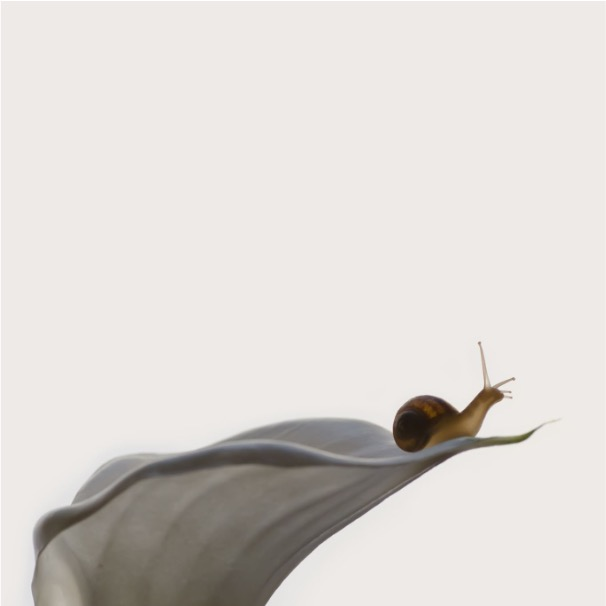
\includegraphics[scale=0.3]{snail.jpg}
		\caption{Example of a Snail}
	\end{figure}
\end{columns}

\end{frame}

%Introduction%
\section{Introduction}
\begin{frame}
	\frametitle{Introduction}

	\begin{itemize}
		\item Bella and Grandmother talking about snail
	\end{itemize}

	\begin{description}
	\item[\textcolor{red}{C}] Bella, the child learning English
	\item[G] Her grandmother, caregiver and MKO
	\end{description}

	\begin{itemize}
		\item Bella well into the telegraphic stage
		\item About 5 months ahead
	\end{itemize}
\end{frame}

\begin{frame}
	\frametitle{Introduction}
	
	\begin{displayquote}
		We are storytelling creatures, and as children we acquire language to tell those stories that we have inside us.” - Jerome Bruner	
	\end{displayquote}

\end{frame}

\section{Features of Language}
\subsection{Emerging Subsystems}
\begin{frame}
	\frametitle{Emerging Subsystems}
	\begin{itemize}
		\item Bella's Developmental Stage $\rightarrow$ well into telegraphic
		\item Coherent utterances, but missing function words/morphemes
	\end{itemize}
	\noindent\rule{\textwidth}{1pt}
	
	\centering
	Typical Utterances:
	\vspace{2mm}
	\begin{columns}
		\column{0.5\textwidth}
			\centering
			\begin{displayquote}
				"Where daddy?"
			\end{displayquote}

		\column{0.5\textwidth}
			\centering
			\begin{displayquote}
				"What that?
			\end{displayquote}
	\end{columns}

	
\end{frame}

%Lexical and Semantic Perspective%
\begin{frame}
	\frametitle{Emerging Subsystems - Lexical and Semantic Perspective}
	
	\begin{itemize}
		\item Actively asking where questions
	\end{itemize}
	\begin{description}
	\item[\textcolor{red}{C}] Where \textipa{[nʌdə sneɪjəl]}
	\end{description}
\end{frame}

\subsection{Supported Theories}
%Carer Strategies%

\section{The Subsystems}
\subsection{Phonological Processes}
\subsection{Lexicology}
\subsection{Morphology}
\subsection{Semantics}
\subsection{Syntax}
\subsection{Discourse}

\section{Conclusion}

\end{document}
